\documentclass{article}
\usepackage{graphicx} % Required for inserting images
\usepackage{caption}
\usepackage{subcaption}
\usepackage{amsmath}
\usepackage[left=2cm, right=2cm, top=2cm, bottom=2cm]{geometry}

\setlength{\parindent}{0pt}

\title{Assignment 1 -- Kalman Filtering}
\author{Esraaj Sarkar Gupta}
\date{February 2026}

\begin{document}

\maketitle

\section{Introduction}
In this assignment, Kalman filtering is implemented on measurements read from an inertial moment unit (IMU). The following tasks are completed in sequence.

\begin{enumerate}
    \item Roll angle estimation is carried out purely using gyroscope integration.
    \item Roll angle estimation is carried out purely using accelerometer integration.
    \item The Kalman filtering algorithm is implemented.
\end{enumerate}

\section{Physical and Algorithmic Mathematics}
In this section the physics and the algorithms utilized in completing the tasks of this assignment are discussed.

\subsection{Roll Angle Estimation using Purely Gyroscope Data}
The IMU has been programmed to return gyroscope data in the units of \textit{degrees per second} (DPS). These raw measurements are first converted to rad/s using the formula $\omega_{x,k} = \text{dps}_{x,k} \frac{\pi}{180}$, for an angular velocity $\omega$ with an axis of rotation $x$ at the discrete time $k$. The roll angle evolves as

\begin{equation}
    \dot\phi_x(t) = \omega_x(t).
\end{equation}

Electronic gyroscopes are prone to both systemic biases $b_k$ and noise $\eta_k$. Since the roll angle is estimated as a rolling integral of the angular velocity, the systemic error grows linearly with time, and the noise error grows with the square root of time.

\begin{equation}
    e = bt +  \int_0^t \eta(\tau) d\tau
\end{equation}

\subsection{Roll Angle Estimation using Purely Accelerometer Readings}
In order to estimate the roll angle(s) from accelerometer readings, we apply a sequence of 3D rotation matrices to project the static gravity vector onto the sensor's body frame, allowing us to isolate the specific angles of rotation mathematically.\\
\\
Consider the device at a state $\ddot{\mathbf{X}} = 0$. In the world frame, the gravity vector is given by

\begin{equation}
    G = \begin{pmatrix}
        0 \\
        0 \\
        g
    \end{pmatrix}
\end{equation}
and is shared by the device if the basis of the device is superimposed with the world basis. In order to rotate this matrix in the 3D space, the gravity vector is multiplied by the Pitch $\theta$ and Roll Matrices $\phi$.\\
\\

\textbf{Pitch Matrix} ($R_y$):
\begin{equation}
R_y(\theta) = 
\begin{bmatrix} 
\cos\theta & 0 & -\sin\theta \\ 
0 & 1 & 0 \\ 
\sin\theta & 0 & \cos\theta 
\end{bmatrix}
\end{equation}

\textbf{Roll Matrix} ($R_x$):
\begin{equation}
R_x(\phi) = 
\begin{bmatrix} 
1 & 0 & 0 \\ 
0 & \cos\phi & \sin\phi \\ 
0 & -\sin\phi & \cos\phi 
\end{bmatrix}
\end{equation}

To find the theoretical acceleration measured on each axis ($A_x$, $A_y$, $A_z$), we multiply the matrices against the gravity vector:

\begin{equation}
\begin{bmatrix} 
A_x \\ 
A_y \\ 
A_z 
\end{bmatrix} 
= R_x(\phi) R_y(\theta) 
\begin{bmatrix} 
0 \\ 
0 \\ 
g 
\end{bmatrix}
\end{equation}

This results the following equations.

\begin{equation}
A_x = -g\sin\theta
\end{equation}

\begin{equation}
A_y = g\cos\theta\sin\phi
\end{equation}

\begin{equation}
A_z = g\cos\theta\cos\phi
\end{equation}

Algebraically isolating the roll gives us the final expression

\begin{equation}
\theta = \text{arctan2}\left(-A_x, \sqrt{A_y^2 + A_z^2}\right).
\end{equation}

\subsection{Kalman Filtering}
The discrete system can be described with a scalar

\begin{equation}
    \phi_{K+1} = \phi_k + \omega_kT_s + w_k
\end{equation}

where $\phi_k$ is the roll angle at $k$, $\omega_k$ is the measured angular velocity, $T_s$ is the sampling time and $w_k$ is the process noise. The measurement model can be described by the scalar equation

\begin{equation}
    \phi_{\text{acc}, k} = \theta_k + v_k
\end{equation}

where $v_k$ is the measurement noise.\\
\\

The \textit{A Priori} estimate is given by the expression

\begin{equation}
    \hat\phi_{k+1|k} = \hat\phi_{k|k} + T_s\omega_k
\end{equation}

where $\hat\phi_{k+1|k}$ is the \textit{a priori} predicted angle for the new time step, and $\hat\phi_{k|k}$ is the final, corrected angle from the previous step. The state variance propagates with time, governed by the equation

\begin{equation}
\hat{\Sigma}_{k+1|k} = \hat{\Sigma}_{k|k} + T_{s}^{2}\sigma_{w}^{2}
\end{equation}

where $\hat{\Sigma}_{k+1|k}$ is the \textit{a priori} predicted variance, representing the uncertainty of the estimate before the measurement is incorporated. The term $\hat{\Sigma}_{k|k}$ denotes the \textit{a posteriori} variance from the previous time step, and $\sigma_{w}^{2}$ is the process noise variance, which accounts for the accumulation of error and drift inherent in the gyroscope measurements over the sampling interval $T_s$.\\
\\

Once the \textit{a priori} estimate is established, the measurement from the accelerometer is used to compute the Kalman gain, which dictates the weighting between the predicted state and the noisy observation. The Kalman gain $K$ is computed as:

\begin{equation}
K = \frac{\hat{\Sigma}_{k+1|k}}{\hat{\Sigma}_{k+1|k} + T_{s}^{2}\sigma_{v}^{2}}
\end{equation}

where $\sigma_{v}^{2}$ is the measurement noise variance. This gain is then utilized to update the state estimate to its \textit{a posteriori} form:

\begin{equation}
\hat{\phi}_{k+1|k+1} = \hat{\phi}_{k+1|k} + K (\phi_{\text{acc},k+1} - \hat{\phi}_{k+1|k})
\end{equation}

The term $(\phi_{\text{acc},k+1} - \hat{\phi}_{k+1|k})$ is known as the residual or innovation, representing the discrepancy between the measured angle and the predicted angle. Finally, the state variance is updated to reflect the reduction in uncertainty provided by the measurement:

\begin{equation}
\hat{\Sigma}_{k+1|k+1} = (1 - K) \hat{\Sigma}_{k+1|k}
\end{equation}

This recursive process ensures that the estimate remains stable over time, effectively utilizing the short-term precision of the gyroscope while correcting for its long-term drift using the absolute reference of the accelerometer.

\section{Observations}

\subsection{Systemic Biases}
It is evident from observing measurements from the resting device that readings clearly have systemic biases. This is especially obvious when examining the $a_z$ value. One expects $a_z \approx 9.8$, whereas the device measurement was closer to $9.5$. Since $\phi$ is estimated from integrating $\omega$, the gyroscope errors compound linearly with time, as depicted in Fig.\ref{fig:systemic_bias}.

\begin{figure}[htbp]
     \centering
     \begin{subfigure}[b]{0.45\textwidth}
         \centering
         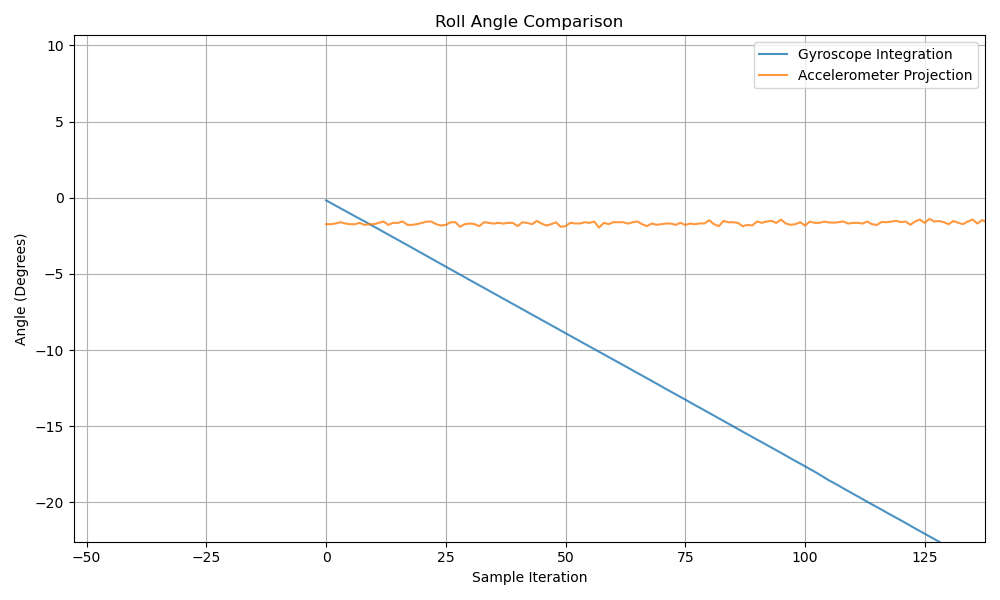
\includegraphics[width=\textwidth]{raw_results/systemic_bias.png}
         \caption{Bias in Device Measurements}
         \label{fig:systemic_bias}
     \end{subfigure}
     \hfill
     \begin{subfigure}[b]{0.45\textwidth}
         \centering
         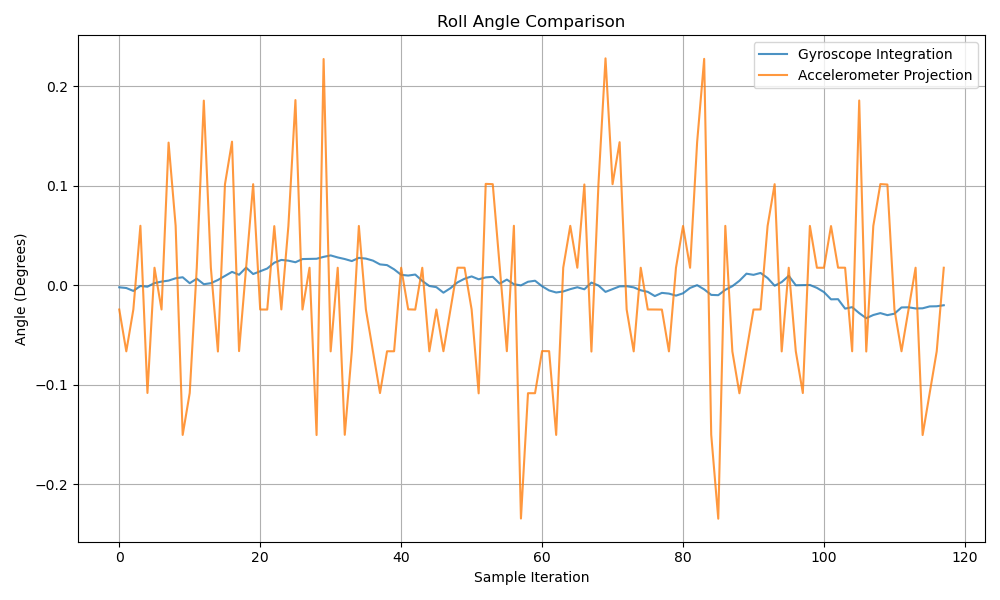
\includegraphics[width=\textwidth]{raw_results/bias_correction.png}
         \caption{}
         \label{fig:bias_correction}
     \end{subfigure}
        \caption{Errors in Device Measurements}
        \label{fig:errors}
\end{figure}



This error is corrected for by including a "burn-in" period, during which the device is allowed to rest. Measurements from the idle device are averaged for all columns and subtracted with the expected values (all zero apart from $a_z$). The bias for each column is subsequently subtracted from every reading during the "main" cycle proceeding the burn-in cycles. It is evident from Fig.\ref{fig:bias_correction} that this is effective.

One may still observe aliasing if the device is perturbed faster than its Nyquist Limit. This is demonstrated in Fig. \ref{fig:aliasing}.

\begin{figure}[h!]
    \centering
    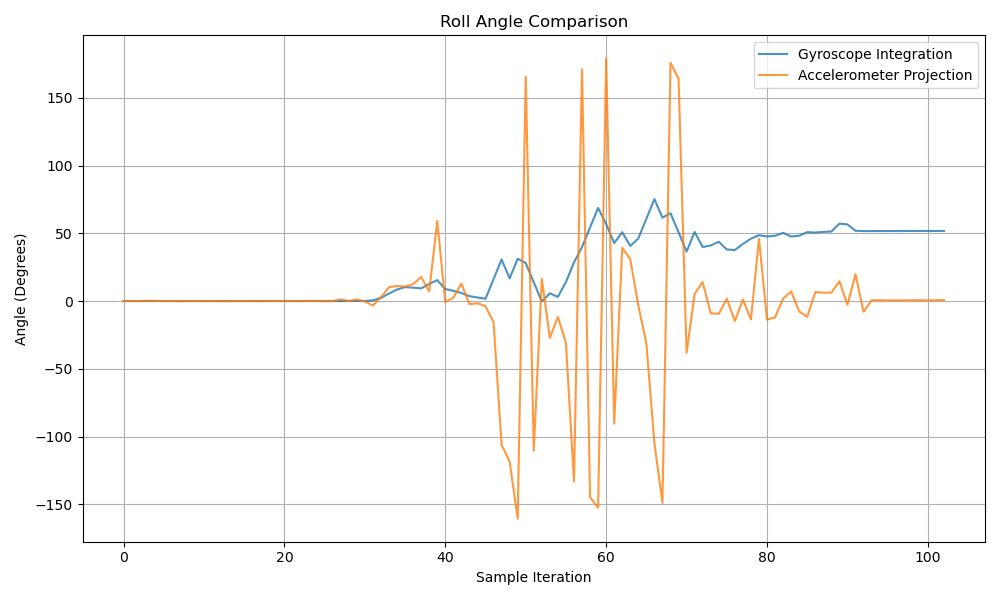
\includegraphics[width=0.5\linewidth]{raw_results/errors_compound.png}
    \caption{Aliasing}
    \label{fig:aliasing}
\end{figure}

\subsection{Vanilla Roll Angle Estimators}

In order to rest the sensors post-calibration, the device is simply rotated 90 degrees. From Fig.\ref{fig:90_degrees_compare} it is seen that the gyroscope tends to under-predict the true angle. The possibility of this being an artifact is ruled out by Fig.\ref{fig:90_degress_nocorrection} where the bias correction has been removed -- this is visible from a subtle drift in the gyroscope measurements.

\begin{figure}[htbp]
     \centering
     \begin{subfigure}[b]{0.45\textwidth}
         \centering
         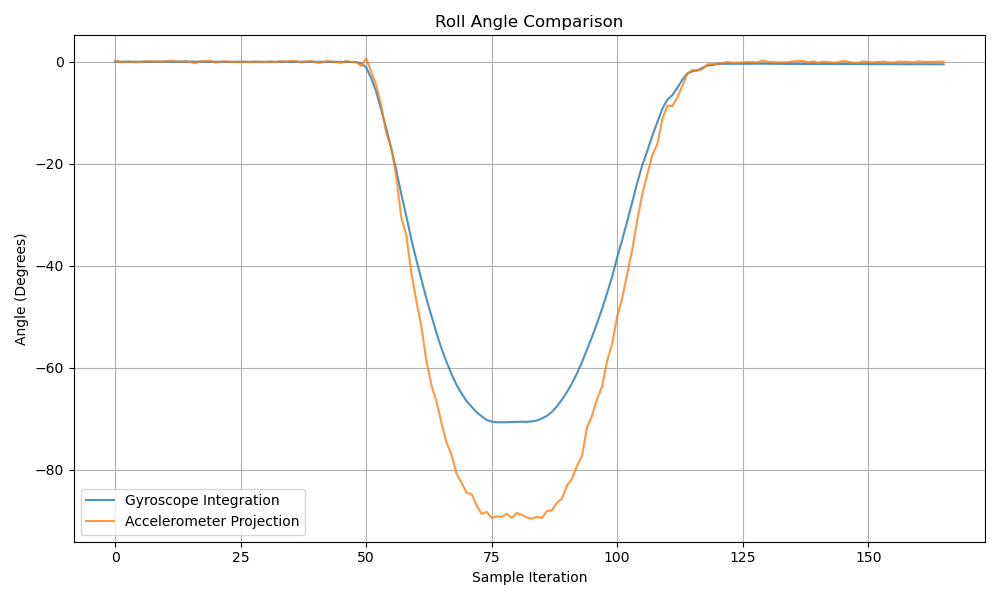
\includegraphics[width=\textwidth]{raw_results/90_degress.png}
         \caption{90 Degree Rotation}
         \label{fig:90_degress}
     \end{subfigure}
     \hfill
     \begin{subfigure}[b]{0.45\textwidth}
         \centering
         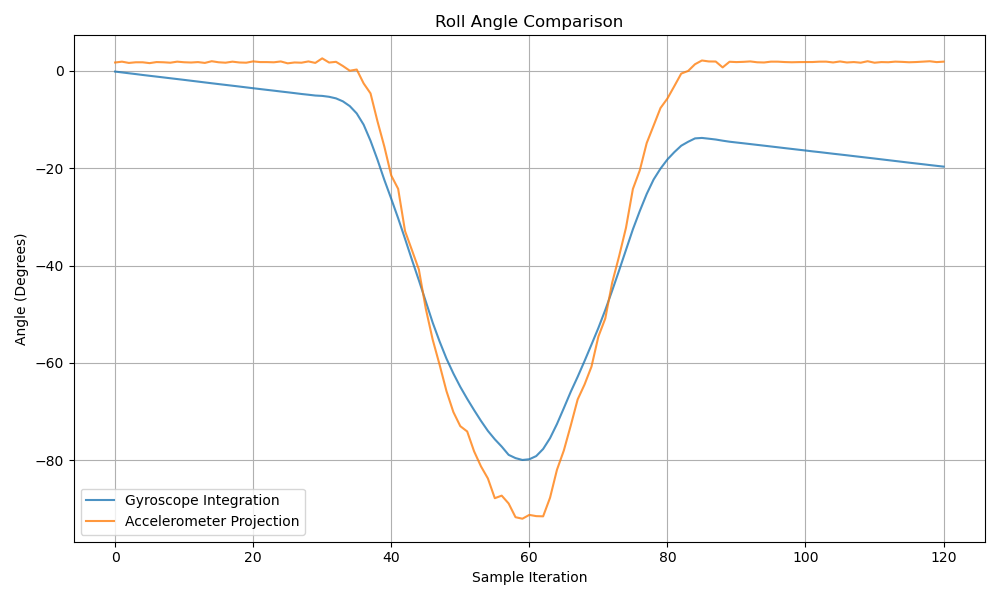
\includegraphics[width=\textwidth]{raw_results/90_degress_nocorrection.png}
         \caption{90 Degrees Rotation without Bias Correction}
         \label{fig:90_degress_nocorrection}
     \end{subfigure}
        \caption{Comparing Gyroscopic and Accelerometric Measurements}
        \label{fig:90_degrees_compare}
\end{figure}

 The roll angle given by the accelerometer measurements and the gyroscope measurements are observed to have a Pearson's correlation coefficient of $r = 0.986$.
 
\begin{figure}[h!]
    \centering
    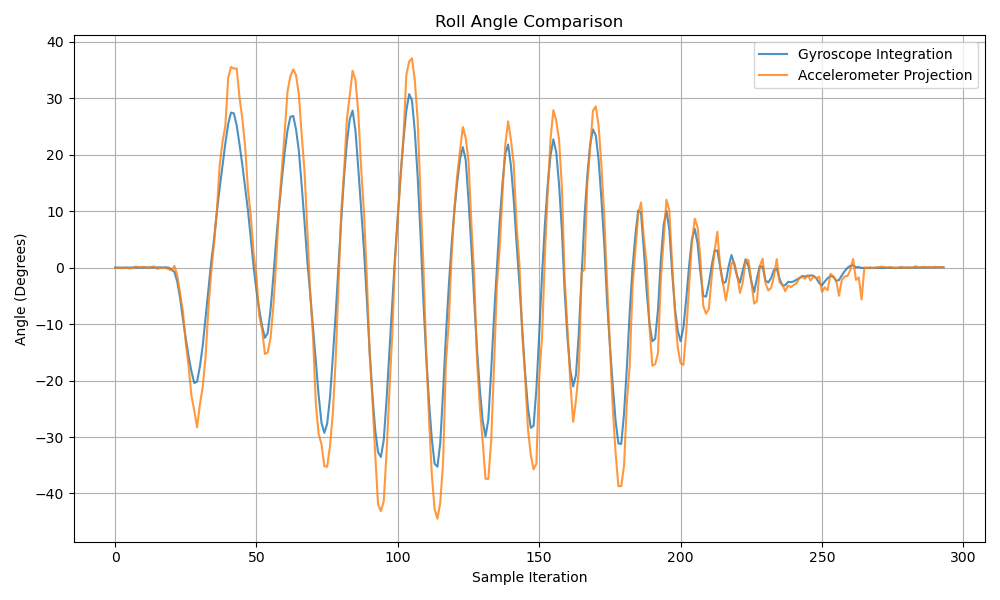
\includegraphics[width=0.5\linewidth]{raw_results/correlation986.png}
    \caption{Observed Correlation $r = 0.986$}
    \label{fig:correlation}
\end{figure}

Another interesting observation is how observations from $\omega$ are unbounded due to the compounding nature of the estimator, a result of the integral. However, since the accelerometer uses \texttt{arctan2} to estimate $\phi$, it is bounded to the limits $[-180, 180]$. A 360 rotation is done to demonstrate this in Fig.\ref{fig:360}.

\begin{figure}[h!]
    \centering
    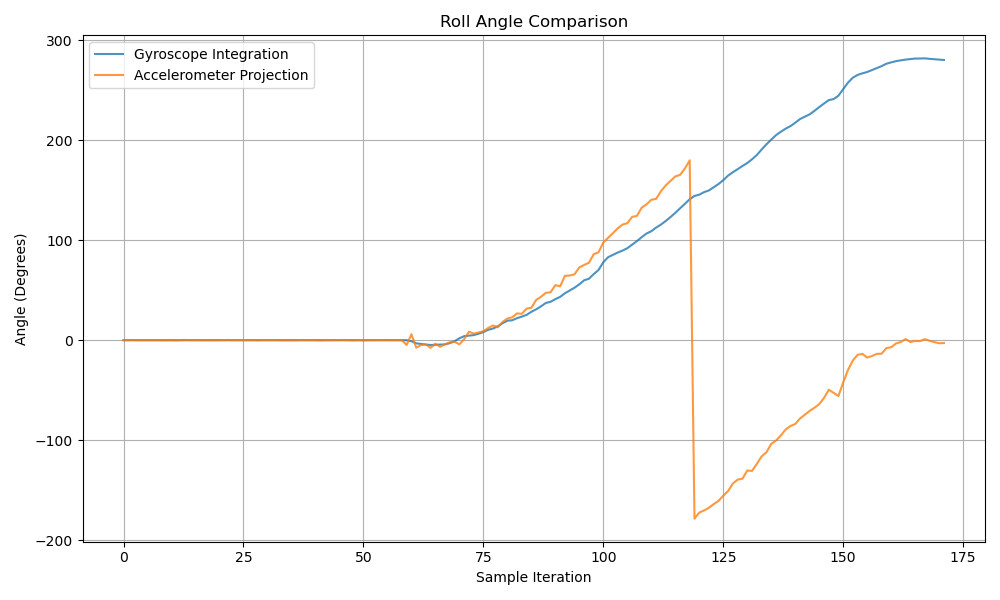
\includegraphics[width=0.5\linewidth]{raw_results/360_sense.png}
    \caption{360 Degree Rotation}In
    \label{fig:360}
\end{figure}

\subsection{Kalman Filtered Roll Angle Estimators}

The stability of the filter is further evidenced in Fig. \ref{fig:kalman_correlation}, where the fused estimate exhibits high correlation with the underlying signal while significantly attenuating the high-frequency noise inherent in the raw accelerometer projection.

\begin{figure}[htbp]
     \centering
     \begin{subfigure}[b]{0.45\textwidth}
         \centering
         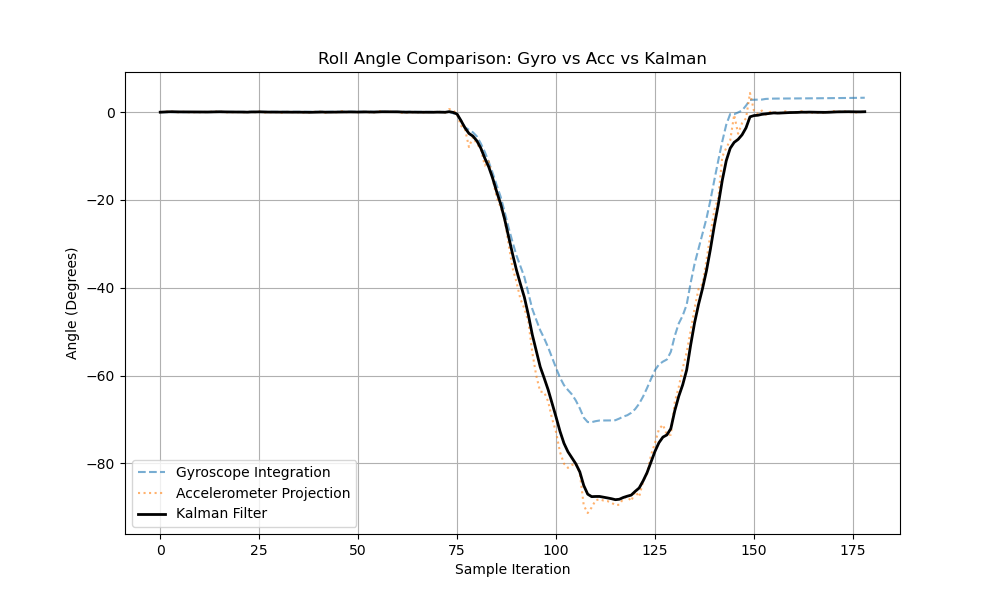
\includegraphics[width=\textwidth]{kalman_results/kalman90.png}
         \caption{90 Degree Rotation}
         \label{fig:}
     \end{subfigure}
     \hfill
     \begin{subfigure}[b]{0.45\textwidth}
         \centering
         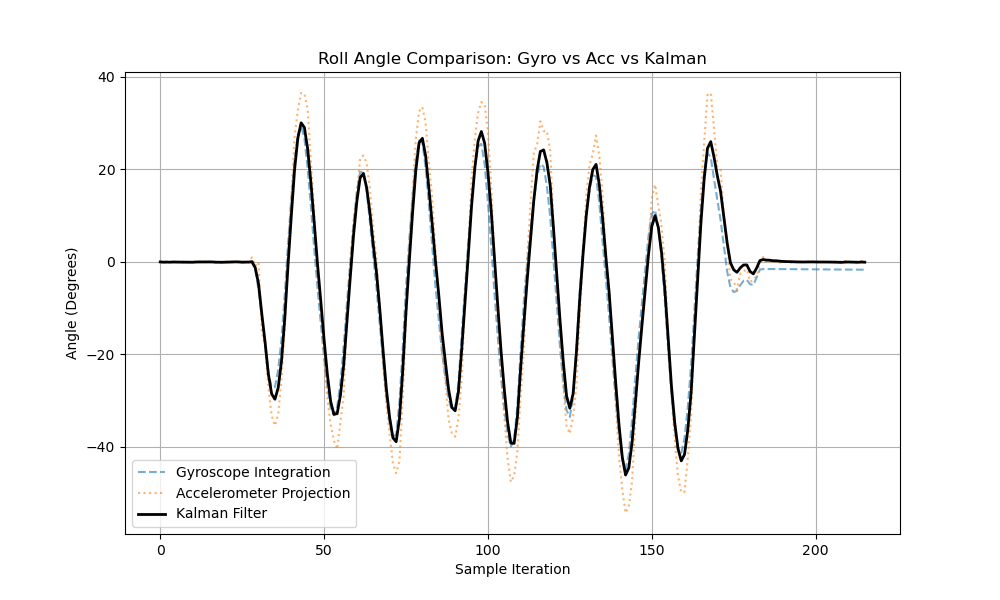
\includegraphics[width=\textwidth]{kalman_results/kalman_correlation.png}
         \caption{Rolling}
         \label{fig:kalman_correlation}
     \end{subfigure}
        \caption{Kalman Filter Results}
        \label{fig:}
\end{figure}

A critical observation is the filter's behavior when the two models diverge. In the $360^{\circ}$ rotation maneuver, gyroscopic drift and integration errors cause the pure-integration estimate to deviate significantly from the true orientation. However, the Kalman filter correctly identifies the accelerometer projection as the absolute reference.

\begin{figure}[h!]
    \centering
    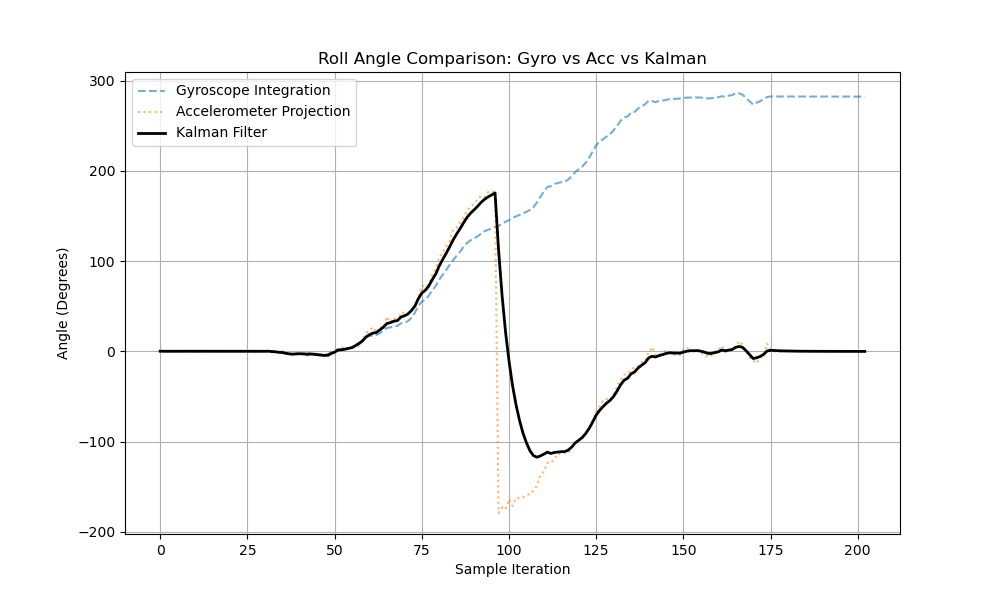
\includegraphics[width=0.5\linewidth]{kalman_results/Figure_1kalman360.png}
    \caption{Behavior as Signals Diverge}
    \label{fig:placeholder}
\end{figure}

\subsection{Parameter Tuning}
When the measurement noise variance $\sigma_v^2$ is set to a low value, the Kalman filter places high trust in the accelerometer data. It is observed that the resulting estimate tracks the accelerometer projection very closely, offering high responsiveness and minimal phase lag during rapid movements. However, this high sensitivity also causes the estimate to incorporate significant high-frequency noise and mechanical vibrations, leading to a "jittery" output that lacks smoothness. Conversely, when $\sigma_v^2$ is high, the filter assumes the accelerometer is unreliable. In this state, the output becomes exceptionally smooth as the filter relies more on the integrated gyroscope prediction, though this leads to a noticeable "lag" where the estimate takes longer to catch up to the true physical orientation.

\begin{figure}[htbp]
     \centering
     \begin{subfigure}[b]{0.45\textwidth}
         \centering
         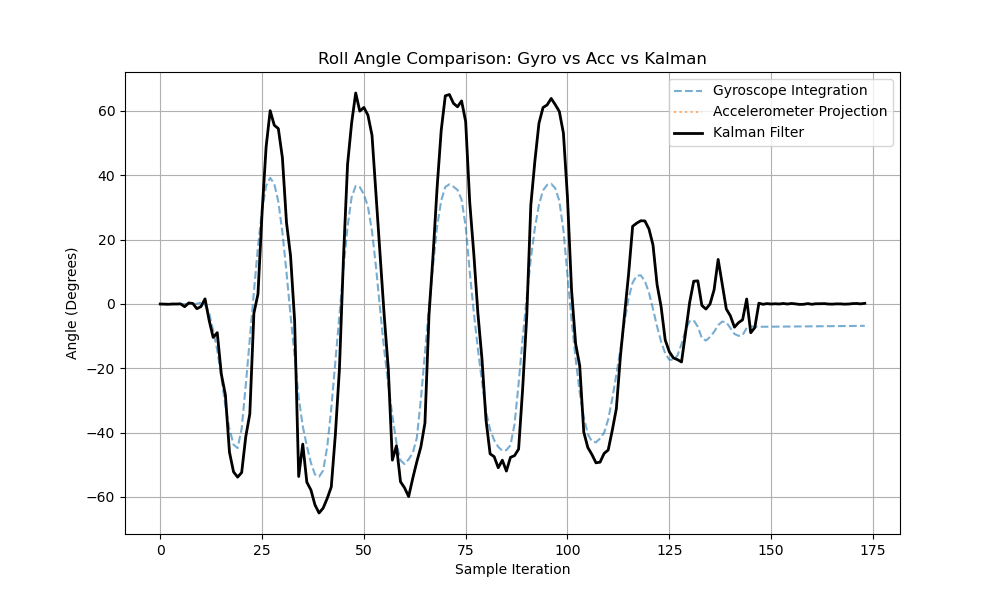
\includegraphics[width=\textwidth]{param_play/sv0001.png}
         \caption{$\sigma_v = 0.0001$}
         \label{fig:}
     \end{subfigure}
     \hfill
     \begin{subfigure}[b]{0.45\textwidth}
         \centering
         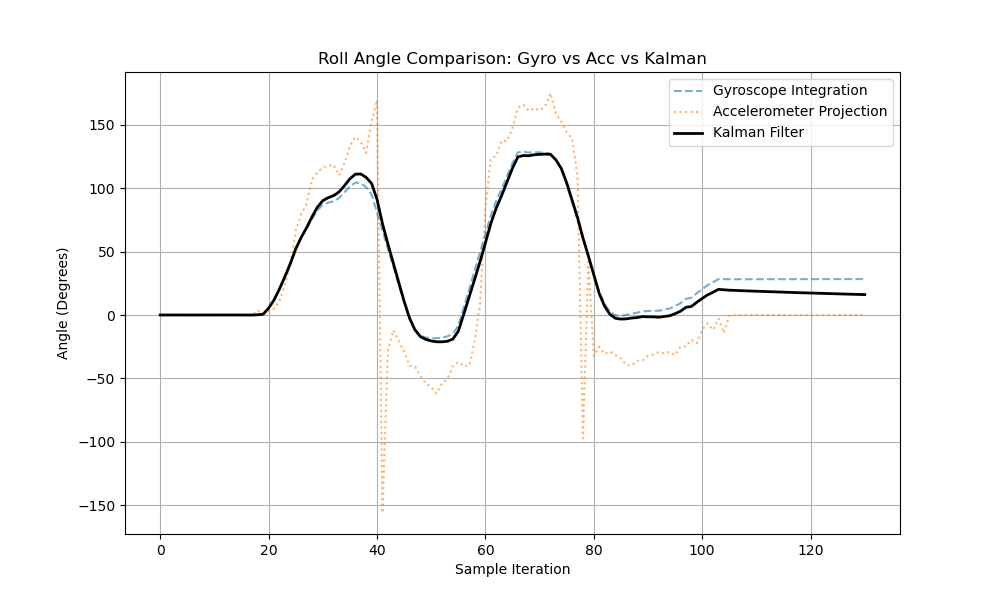
\includegraphics[width=\textwidth]{param_play/sv50dot00_lag.png}
         \caption{$\sigma_v = 50$, observable lag}
         \label{fig:}
     \end{subfigure}
        \caption{Tuning $\sigma_v$}
        \label{fig:}
\end{figure}

The process noise variance $\sigma_w^2$ represents the uncertainty added to the state estimate by the gyroscope integration at each time step. When $\sigma_w^2$ is low, the filter assumes the gyroscope is a near-perfect model of the system's dynamics. This results in a very stable and smooth signal.

\begin{figure}[htbp]
     \centering
     \begin{subfigure}[b]{0.45\textwidth}
         \centering
         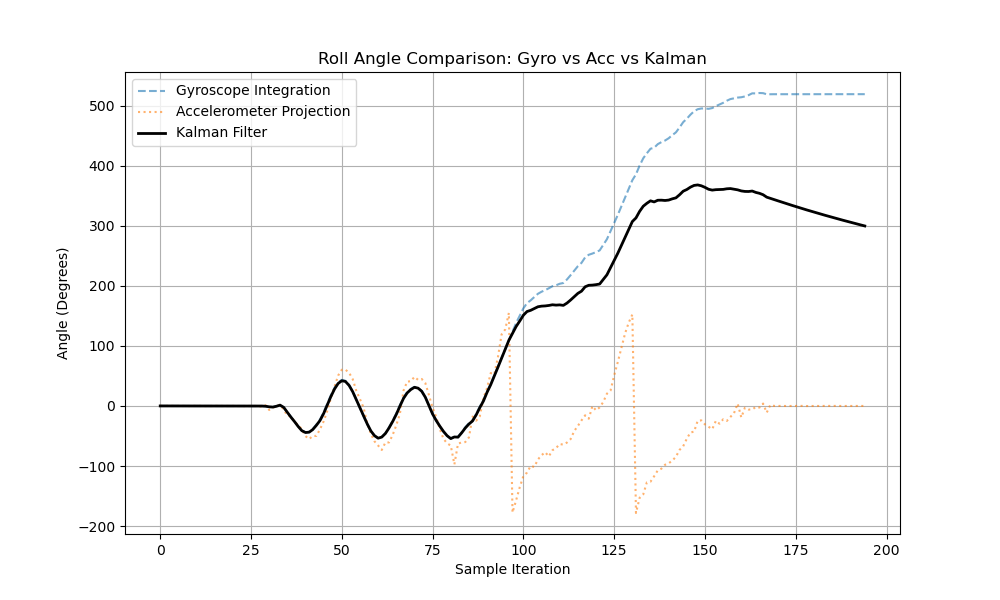
\includegraphics[width=\textwidth]{param_play/sw0001.png}
         \caption{$\sigma_\omega = 0.0001$}
         \label{fig:}
     \end{subfigure}
     \hfill
     \begin{subfigure}[b]{0.45\textwidth}
         \centering
         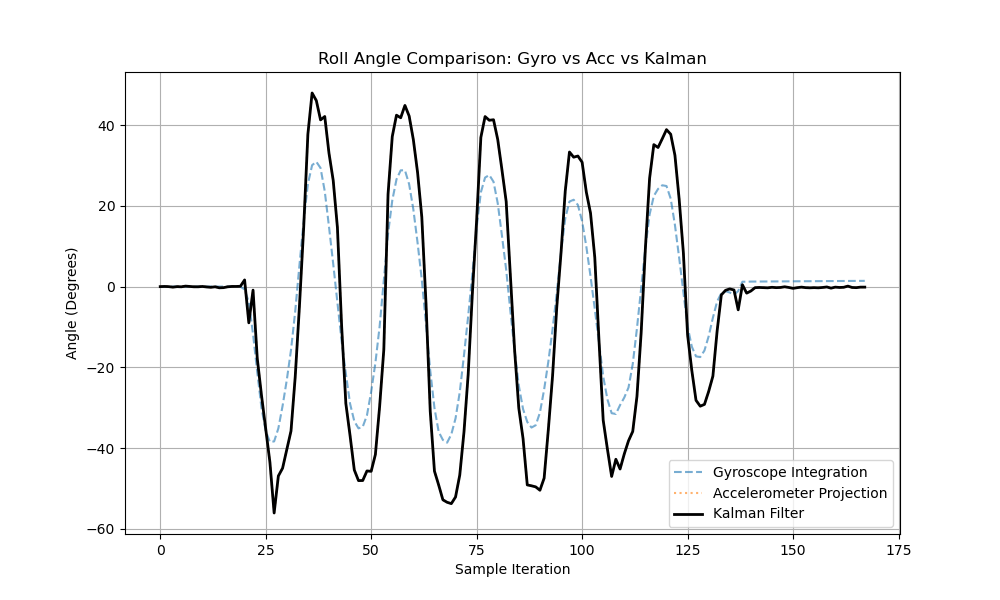
\includegraphics[width=\textwidth]{param_play/sw_40dot.png}
         \caption{$\sigma_\omega = 40$}
         \label{fig:}
     \end{subfigure}
        \caption{Tuning $\sigma_\omega$}
        \label{fig:}
\end{figure}

One may further emphasize the effect that a low $\sigma_\omega$ by observing Fig.\ref{fig:unphys} where a physically impossible system is simulated (by messing with the I$^2$C communication protocol of the hardware setup). Despite such a massive difference between the gyroscopic and accelerometric measurements, the Kalmn Filtered signal follows the accelerometer signal almost entirely.

\vfill

\begin{figure}[h!]
    \centering
    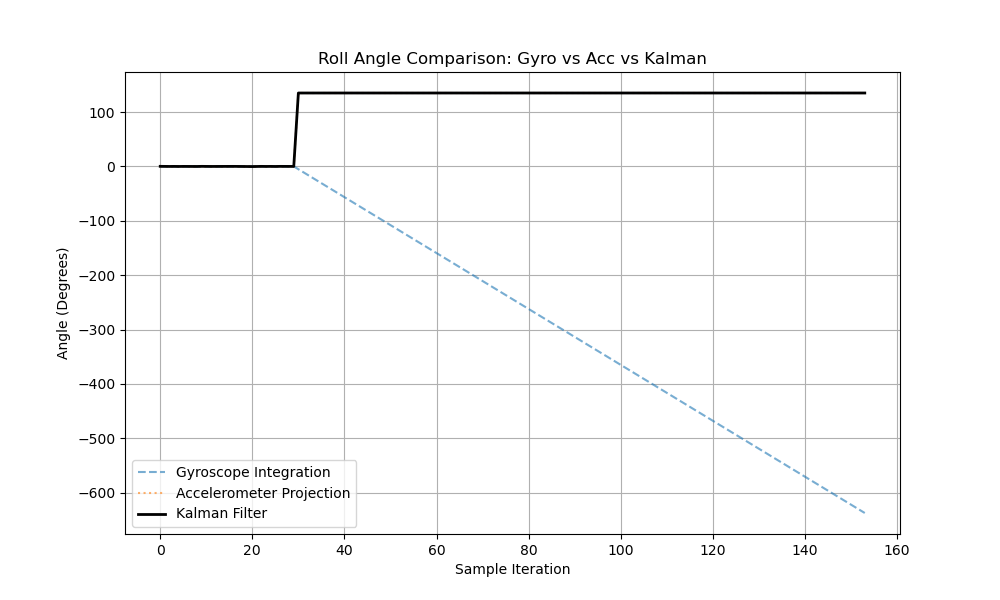
\includegraphics[width=0.5\linewidth]{param_play/sw40_unphysical.png}
    \caption{Impossible System, $\sigma_\omega = 0.0001$}
    \label{fig:unphys}
\end{figure}

It is observed that the sampling interval $T_s$ plays a critical role in the reliability of the gyroscope integration. Because the system only takes snapshots of the angular velocity every 50ms, any high-frequency movement that happens between those samples is effectively lost. This violates the Nyquist limit for the system. The accelerometer does not exhibit this same type of compounding drift, since it provides an absolute reference to gravity at every sample.






\end{document}

The initial state variance $\hat{\Sigma}_0$ dictates the filter's convergence behavior at the beginning of a measurement cycle. It is observed that when $\hat{\Sigma}_0$ is initialized to a low value, the filter begins with high confidence in its initial state. If there is a discrepancy between the initialized angle and the actual orientation of the device, the estimate "stubbornly" and slowly crawls toward the correct value over several iterations. In contrast, when $\hat{\Sigma}_0$ is set to a very high value, the filter treats its initial position as unknown. This leads to an immediate "snap" or jump in the estimate as soon as the first accelerometer measurement is processed, as the filter prioritizes the absolute reference to resolve its high initial uncertainty.


\begin{figure}[htbp]
     \centering
     \begin{subfigure}[b]{0.45\textwidth}
         \centering
         \includegraphics[width=\textwidth]{}
         \caption{}
         \label{fig:}
     \end{subfigure}
     \hfill
     \begin{subfigure}[b]{0.45\textwidth}
         \centering
         \includegraphics[width=\textwidth]{}
         \caption{}
         \label{fig:}
     \end{subfigure}
        \caption{}
        \label{fig:}
\end{figure}
